\documentclass[11pt]{article}

\usepackage[review]{acl}

\usepackage{times}
\usepackage{latexsym}
\usepackage[T1]{fontenc}
\usepackage[utf8]{inputenc}
\usepackage{microtype}
\usepackage{graphicx}
\usepackage{amsmath}
\usepackage{amssymb}
\usepackage{booktabs}
\usepackage{tikz}
\usepackage{pgfplots}
\pgfplotsset{compat=1.18}
\usetikzlibrary{positioning,arrows.meta,calc}
\definecolor{BrandA}{HTML}{4C4CA8}
\definecolor{BrandB}{HTML}{1F7A6B}
% Figures for "Same Text, Different Transitions".
% Every value here is recomputed by artifact/reproduce.sh.

% Figure 1
% The phenomenon: one root, two histories, one rendering, two outcomes.
\newcommand{\FigMechanism}{%
\begin{figure}[t]\centering
\resizebox{\columnwidth}{!}{%
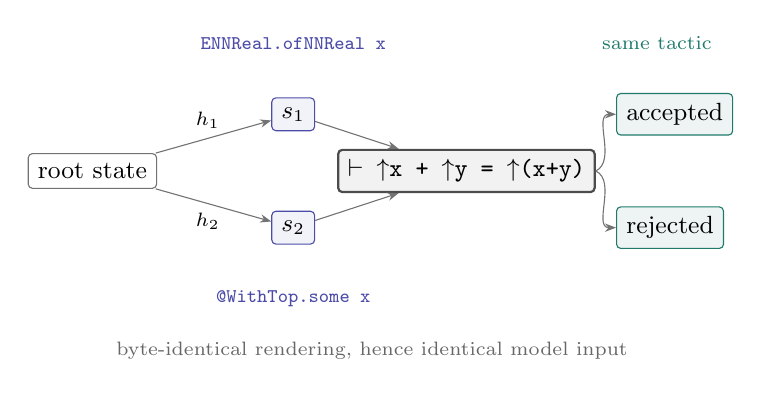
\begin{tikzpicture}[
  font=\small,
  box/.style={draw=black!55,rounded corners=1.5pt,inner sep=3.5pt,
              align=center,fill=white},
  hid/.style={box,draw=BrandA,fill=BrandA!7},
  obs/.style={box,draw=black!70,fill=black!5,thick},
  res/.style={box,draw=BrandB,fill=BrandB!8},
  ar/.style={-{Stealth[length=4pt]},draw=black!55},
]
\node[box] (root) at (0,0) {root state};
\node[hid] (sa) at (2.55,0.72) {$s_1$};
\node[hid] (sb) at (2.55,-0.72) {$s_2$};
\node[obs] (obs) at (4.75,0) {\texttt{$\vdash$ $\uparrow$x + $\uparrow$y = $\uparrow$(x+y)}};
\node[res,anchor=west] (oa) at (6.65,0.72) {accepted};
\node[res,anchor=west] (ob) at (6.65,-0.72) {rejected};

\draw[ar] (root) -- node[above,font=\scriptsize,pos=.45] {$h_1$} (sa);
\draw[ar] (root) -- node[below,font=\scriptsize,pos=.45] {$h_2$} (sb);
\draw[ar] (sa) -- (obs); \draw[ar] (sb) -- (obs);
\draw[ar] (obs.east) to[out=25,in=180] (oa.west);
\draw[ar] (obs.east) to[out=-25,in=180] (ob.west);

\node[font=\scriptsize,BrandA,align=center] at (2.55,1.62)
  {\texttt{ENNReal.ofNNReal x}};
\node[font=\scriptsize,BrandA,align=center] at (2.55,-1.62)
  {\texttt{@WithTop.some x}};
\node[font=\scriptsize,black!60,align=center] at (3.55,-2.28)
  {byte-identical rendering, hence identical model input};
\node[font=\scriptsize,BrandB,align=center,anchor=west] at (6.35,1.62)
  {same tactic};
\end{tikzpicture}}
\caption{Observation aliasing. Two histories from one root reach states that
differ only in elaborated structure the printer collapses; the rendering, and
therefore the entire input supplied to the evaluated state-only generators, is
byte-identical, yet the same tactic is accepted on one and rejected on the
other.}
\label{fig:mechanism}
\end{figure}}

% Figure 2
% Logical evidence ladder with distinct denominators presented separately.
\newcommand{\FigEvidence}{%
\begin{figure}[t]\centering
\resizebox{0.94\columnwidth}{!}{%
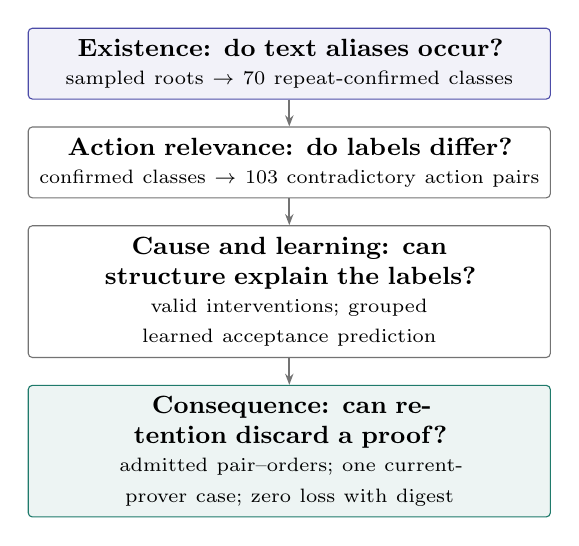
\begin{tikzpicture}[
  font=\small,
  ev/.style={draw=black!55,rounded corners=1.5pt,inner sep=4pt,
             text width=6.35cm,align=center,fill=white},
  ar/.style={-{Stealth[length=4pt]},draw=black!55,thick},
]
\node[ev,draw=BrandA,fill=BrandA!7] (e1) at (0,0)
  {\textbf{Existence: do text aliases occur?}\\[-1pt]\scriptsize sampled roots $\rightarrow$ 70 repeat-confirmed classes};
\node[ev,below=0.34cm of e1] (e2)
  {\textbf{Action relevance: do labels differ?}\\[-1pt]\scriptsize confirmed classes $\rightarrow$ 103 contradictory action pairs};
\node[ev,below=0.34cm of e2] (e3)
  {\textbf{Cause and learning: can structure explain the labels?}\\[-1pt]\scriptsize valid interventions; grouped learned acceptance prediction};
\node[ev,draw=BrandB,fill=BrandB!8,below=0.34cm of e3] (e4)
  {\textbf{Consequence: can retention discard a proof?}\\[-1pt]\scriptsize admitted pair--orders; one current-prover case; zero loss with digest};
\draw[ar] (e1) -- (e2); \draw[ar] (e2) -- (e3); \draw[ar] (e3) -- (e4);
\end{tikzpicture}}
\caption{Conceptual evidence spine. Each arrow asks a separate question and
uses the denominator printed beneath it. Population incidence, contradictory
actions, structural learnability, and conditional search loss are estimated
separately.}
\label{fig:evidence}
\end{figure}}

% Figure 3
% Intervention: construction, validity gate, and per-family result.
\newcommand{\FigIntervention}{%
\begin{figure*}[t]\centering
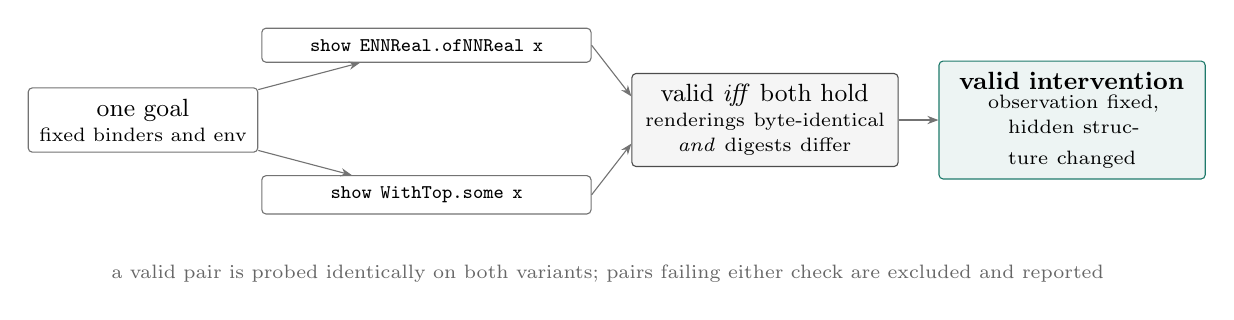
\begin{tikzpicture}[
  font=\small,
  b/.style={draw=black!55,rounded corners=1.5pt,inner sep=4pt,align=center,fill=white},
  gate/.style={b,draw=black!70,fill=black!4},
  ok/.style={b,draw=BrandB,fill=BrandB!8},
  no/.style={b,draw=black!45,fill=black!7},
  ar/.style={-{Stealth[length=4pt]},draw=black!55},
]
% Four stages fit the two-column width. The footnote line states the probing
% step. The two variant boxes
% share a text width so their edges align and the gate arrows stay symmetric.
\node[b] (goal) at (0,0) {one goal\\[-2pt]\scriptsize fixed binders and env};
\node[b,text width=3.9cm] (a)  at (3.6,0.95) {\scriptsize\texttt{show ENNReal.ofNNReal x}};
\node[b,text width=3.9cm] (bb) at (3.6,-0.95) {\scriptsize\texttt{show WithTop.some x}};
\node[gate,text width=3.1cm] (gate) at (7.9,0)
  {\centering valid \emph{iff} both hold\\[1pt]
   \scriptsize renderings byte-identical\\[-2pt]
   \emph{and} digests differ};
\node[ok,text width=3.1cm] (valid) at (11.8,0)
  {\centering\textbf{valid intervention}\\[-1pt]
   \scriptsize observation fixed,\\[-2pt]hidden structure changed};
\draw[ar] (goal) -- (a); \draw[ar] (goal) -- (bb);
\draw[ar] (a.east) -- ($(gate.west)+(0,0.30)$);
\draw[ar] (bb.east) -- ($(gate.west)+(0,-0.30)$);
\draw[ar] (gate) -- (valid);
\node[font=\scriptsize,black!60,align=center] at (5.9,-1.95)
  {a valid pair is probed identically on both variants;
   pairs failing either check are excluded and reported};
\end{tikzpicture}

\vspace{3pt}
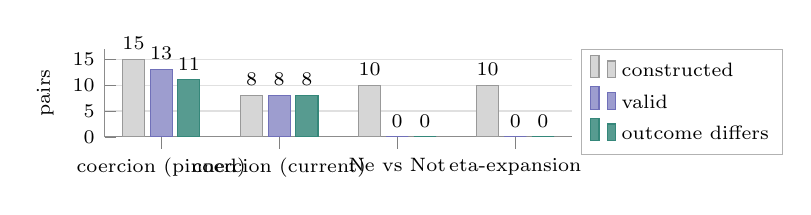
\begin{tikzpicture}
\begin{axis}[
  width=0.62\textwidth, height=2.7cm,
  ybar, ymin=0, ymax=17,
  bar width=8pt, enlarge x limits=0.16,
  symbolic x coords={coercion (pinned),coercion (current),Ne vs Not,eta-expansion},
  xtick=data, tick label style={font=\scriptsize},
  ylabel={pairs}, ylabel style={font=\scriptsize},
  axis lines*=left, axis line style={draw=black!45},
  ymajorgrids, grid style={black!12},
  legend style={font=\scriptsize,at={(1.02,1.0)},anchor=north west,draw=black!30},
  legend cell align=left,
  nodes near coords, nodes near coords style={font=\scriptsize},
]
\addplot[fill=black!16,draw=black!40] coordinates {
  (coercion (pinned),15) (coercion (current),8) (Ne vs Not,10) (eta-expansion,10)};
\addlegendentry{constructed}
\addplot[fill=BrandA!55,draw=BrandA!80] coordinates {
  (coercion (pinned),13) (coercion (current),8) (Ne vs Not,0) (eta-expansion,0)};
\addlegendentry{valid}
\addplot[fill=BrandB!75,draw=BrandB!90] coordinates {
  (coercion (pinned),11) (coercion (current),8) (Ne vs Not,0) (eta-expansion,0)};
\addlegendentry{outcome differs}
\end{axis}
\end{tikzpicture}
\caption{Rendering-preserving interventions. \textbf{Top:} the construction.
A single \texttt{show} step replaces the goal with a definitionally equal term,
so only the elaborated representation changes; a pair is used only if it passes
both checks. \textbf{Bottom:} outcomes. The construction succeeds for the
coercion family under the pinned stack and, with acceptance-sensitive probes,
on a current Lean and Mathlib, where all 8 pairs are accepted on one variant
and rejected on the other. The other two families yield zero valid pairs
because the printer renders their two spellings differently.}
\label{fig:intervention}
\end{figure*}}


\title{Same Text, Different Transitions:\\
Action Insufficiency in Lean Provers}

\author{Anonymous submission}

\begin{document}
\maketitle

\begin{abstract}
Neural Lean provers commonly condition tactic policies on a pretty-printed
proof state, and some search procedures also use that rendering as node
identity. We test the necessary assumption that the rendering is
\emph{action-sufficient}. Searches over Mathlib produce 70 repeat-verified
alias classes and 103 paired state--tactic observations with identical text and opposite
compiler labels, providing counterexamples to action sufficiency. Controlled
rendering-preserving interventions identify notation-collapsed elaborated
structure as a cause and reproduce the effect on a current Lean and Mathlib.
A small learned acceptance model uses a compact structural channel to recover
member-specific signal across unseen theorems within observed mechanisms. In a
compiler-verified 96-pair stress benchmark, rendering-keyed retention discards
a known available proof in nearly half of uniformly ordered alias arrivals,
whereas a structural identity preserves every proof with 8\% end-to-end
overhead. Blind incidence and broad-search experiments separately measure how
often evaluated policies encounter the demonstrated conditional failure.
\end{abstract}

\section{Introduction}

Neural Lean provers are given a textual rendering and asked to select a tactic.
We show that this interface can map action-distinct states to the same text.
Table~\ref{tab:witness} is one instance: changing
only the order of \texttt{intro h} and \texttt{simp} reaches a common 206-byte
rendering, after which another \texttt{simp} fails on one state and succeeds on
the other. The outcomes repeat on fresh sessions.

\begin{table}[t]\centering\small
\begin{tabular}{@{}lll@{}}
\toprule
 & history & then \texttt{simp} \\
\midrule
$s_1$ & \texttt{intro h; simp} & fails ($\times$3) \\
$s_2$ & \texttt{simp; intro h} & succeeds ($\times$3) \\
\bottomrule
\end{tabular}
\caption{Two states in one Mathlib proof
(\texttt{lintegral\_\allowbreak ofReal\_\allowbreak le\_\allowbreak lintegral\_\allowbreak nnnorm}), reached from a common
ancestor by different tactic sequences. Both render to an identical 206-byte
string; the same tactic, replayed three times per state on fresh sessions,
deterministically fails on one and succeeds on the other.}
\label{tab:witness}
\end{table}

Learned tactic generators for interactive theorem provers now close a
substantial share of held-out library and competition
problems~\cite{polu2020gpt-f,han2022pact,lample2022hypertree,yang2023leandojo,
jiang2023draft}, on benchmarks such as miniF2F~\cite{zheng2022minif2f} and
PutnamBench~\cite{tsoukalas2024putnambench}. Many share one interface
decision: the policy conditions on a pretty-printed rendering of the proof
state, and some best-first search implementations also use that text as the
identity of a search node~\cite{yang2023leandojo,lample2022hypertree}. These
uses assume that the observation identifies the state's response to an action,
a transition-preservation condition required by safe state
abstraction~\cite{givan2003equivalence,li2006towards}. It is also implicit in
learning tactic semantics from observed transitions~\cite{samoylov2025operators,
lamont2025threedprover}. We test that assumption directly.

The issue also has a supervised-learning formulation. When the state rendering
and tactic text are identical but compiler acceptance differs, a text-only
acceptance predictor receives contradictory deterministic labels. The resulting
error cannot be removed by model scale or optimization while the observation
is fixed. This affects tactic-effect prediction, reranking, transition
modeling, imitation learning, dataset construction, and evaluation wherever
the rendered state is treated as a complete conditioning variable.

\FigMechanism
\FigEvidence
The hidden difference in Figure~\ref{fig:mechanism} is sixteen bytes of
elaborated term: \texttt{ENNReal.ofNNReal x} versus
\texttt{@WithTop.some.\{0\} NNReal x}. They are definitionally equal and both
print as \texttt{{\textuparrow}x}, but \texttt{simp}'s syntactic progress test
distinguishes them. We call two such states \emph{observation aliases}.
Figure~\ref{fig:evidence} organizes the evidence by logical implication and
keeps incidence and consequence on their respective denominators. Its arrows
ask distinct questions: whether aliases exist, whether the hidden difference
changes an action, whether structural information explains and predicts the
change, and whether an unsafe retention rule can discard a proof. Evidence for
one arrow does not substitute for the denominator of another.

Over Mathlib~\cite{mathlib2020} in Lean~4~\cite{moura2021lean4} through
LeanDojo~\cite{yang2023leandojo}, we make three contributions:
\begin{enumerate}
\item \textbf{Impossibility.} We give repeat-verified counterexamples to action
sufficiency: 68 natural alias classes contain opposite acceptance labels for
the same tactic, yielding 103 contradictory textual inputs
(\S\ref{sec:formal}--\ref{sec:aliases}). This conclusion is independent of the
frequency with which a current policy encounters an alias.
\item \textbf{Empirical phenomenon.} Controlled interventions identify hidden
elaborated structure as causal. A small acceptance model learns to use a compact
structural channel, with theorem-grouped and mechanism-grouped evaluations
separating interpolation from mechanism transfer
(\S\ref{sec:mechanism}--\ref{sec:utility}).
\item \textbf{Engineering consequence and repair.} A current step-prover and a
96-pair alias-conditioned stress benchmark demonstrate proof loss under unsafe
retention. A structural identity key prevents every controlled loss at modest
cost (\S\ref{sec:search}).
\end{enumerate}
Blind incidence, candidate exposure, and broad paired searches estimate the
separate conditions under which the representational failure affects a search.
Data, harnesses, and per-class outcomes are released.

\section{Problem and scope}
\label{sec:formal}

Let $T(s,a)$ denote the result of executing tactic $a$ at Lean tactic state
$s$, and $\Psi$ the observable outcome (acceptance with a successor, rejection,
or proof closure). Rejection is what the interaction API reports as an error,
including Lean's \texttt{made no progress}, the outcome most of the acceptance
contradictions below take. A policy consumes $\varphi(s)$, the pretty-printed
state; write $s_1 \sim_\varphi s_2$ when $\varphi(s_1)=\varphi(s_2)$.

The observation $\varphi$ is \emph{action-sufficient} if $s_1 \sim_\varphi
s_2$ implies $\Psi(T(s_1,a))=\Psi(T(s_2,a))$ for all $a$. This is a necessary
one-step transition-consistency condition for abstractions such as bisimulation
quotients and MDP homomorphisms~\cite{givan2003equivalence,li2006towards},
which impose still stronger preservation requirements. We test only this
one-step condition; its failure rules the stronger properties out. We
distinguish acceptance, visible successor, and bounded-continuation equivalence
throughout.

\paragraph{Acceptance ambiguity.}
For alias class $C$, some $a$ has $r(s_i,a)\neq r(s_j,a)$, where
$r\in\{0,1\}$ is acceptance. The pair $(\varphi(s),a)$ then
carries contradictory verified labels, and any acceptance predictor conditioned
on it errs on at least $\min(n_0,n_1)/(n_0+n_1)$ of members under the
empirical member distribution. This lower bound applies to prediction of a
specified action. The existence of a common successful tactic is a separate
property.

Thus the corpus supplies compiler-verified contradictory supervision rather
than annotation noise: Lean deterministically validates both labels on restored
executable states. A text-only model can learn the average label distribution
for an aliased input, while member-specific prediction requires an additional
observation channel.

Candidate exposure and a direct model-facing test are reported in
\S\ref{sec:utility}; the main text then evaluates search consequences.

\paragraph{Implementation scope.}
The observation claim is independent of a search implementation. The
search-system claim is narrower: in the evaluated stack LeanDojo's \texttt{TacticState}
compares and hashes on the rendering with the executable handle excluded
(\texttt{compare=False}), and the best-first prover keys nodes on that value,
so $\sim_\varphi$-equivalent nodes merge. LeanDojo-v2 uses Pantograph state
handles and a history stack in its active prover, which avoids this particular
merge. Its model prompt still uses the rendered state without the handle, so
the action-sufficiency result continues to apply to policy conditioning.
Appendix~\ref{app:identity} gives the source and behavioral audits. A merge
costs a proof when the discarded member's
bounded continuation language contains a proof absent from the retained
member's language.

\section{Related work}
\label{sec:related}

\paragraph{Textual proof-state interfaces.}
The rendered-goal convention dates to CoqGym~\cite{yang2019coqgym} and
HOList~\cite{bansal2019holist}. miniCTX~\cite{hu2024minictx} and
retrieval-augmented provers~\cite{yang2023leandojo} show that context beyond
the printed goal improves proving across problems. Our within-theorem members
share the file, declaration, statement, and retrievable premises, so ordinary
file context provides identical information for both members.
LeanDojo~\cite{yang2023leandojo},
Pantograph~\cite{aniva2025pantograph}, and LeanTree~\cite{kripner2025leantree}
define model and search interfaces without testing action sufficiency.

\paragraph{Structural and transition-grounded representations.}
Structural encodings are an established alternative to rendering, from graph
representations of higher-order
logic~\cite{paliwal2020graph} to Graph2Tac~\cite{blaauwbroek2024graph2tac} for
Coq definitions. \citet{samoylov2025operators} represent tactic semantics
through induced state transformations, and
3D-Prover~\cite{lamont2025threedprover} filters candidates by learned
transition representations. \citet{olejniczak2026symmetries} exploit proof-state
symmetries. This work asks a logically prior question: whether the visible state
is sufficient to define the transition that these methods model. Identical
observations with contradictory deterministic transitions show that the answer
can be negative. The same counterexample bounds text-based tactic-equivalence
metrics such as LeanTutor's~\cite{leantutor2025}.

\paragraph{Partial observability and search abstraction.}
Observation aliasing is the classical failure of a policy over observations to
see its transition state~\cite{whitehead1991learning,singh1994learning,
kaelbling1998planning}. Tactic searches deduplicate states, the proof-search
analogue of a transposition table~\cite{zobrist1970hashing}; unsafe merging is
the graph-history interaction problem~\cite{kishimoto2004graph}. Here
elaboration creates the path dependence; game repetition rules are irrelevant.

\section{Failure: search-reachable aliases}
\label{sec:aliases}

\begin{table}[t]\centering\small
\setlength{\tabcolsep}{3.2pt}
\begin{tabular}{@{}lrrr@{}}
\toprule
 & blind & coerc. & struct. \\
\midrule
roots replayed             & 1{,}025 & 1{,}423 & 3{,}882 \\
expandable                 & 644     & 947     & 2{,}553 \\
with reconvergence         & 112     & 234     & 667 \\
rendering-identical classes& 150     & 321     & 893 \\
flagged divergent          & 11      & 50      & 36 \\
repeat-confirmed           & \textbf{3} & \textbf{47} & \textbf{21} \\
new after deduplication    & 3       & 47      & 20 \\
acceptance-ambiguous       & 3       & 46      & 19 \\
contradictory pairs        & 6       & 78      & 19 \\
\bottomrule
\end{tabular}
\caption{Discovery by sampling regime. Only the blind column estimates
incidence; targeted columns provide examples for mechanism analysis. One
cross-regime duplicate leaves 70 unique classes.}
\label{tab:regime}
\end{table}

\paragraph{Method.}
From a root state we expand with a fixed tactic pool augmented by goal-derived
rewrites and record, for every rendering, the set of \emph{canonical} histories
reaching it, where a step joins a history only if it changes the rendering
(Appendix~\ref{app:spec}). Classes reached by two prefix-free canonical
histories are probed: one live state per history in a single session, the same
battery for all members, and every flagged class re-verified on a fresh session
with three repetitions per member. States are read at five levels of printer
explicitness by metaprogram probes through the ordinary interaction API
(Appendix~\ref{app:ladder}); derived digests separate the elaborated goal
($F_{\text{core}}$), the environment ($F_{\text{env}}$), and executable
identity. Configuration: Mathlib \texttt{29dcec07}, Lean \texttt{4.10.0-rc1},
LeanDojo 2.0.2. The structural column combines two targeted sweeps. The second
selected 2{,}400 roots and restored 2{,}234; expansion counts exclude failed
restorations.

Table~\ref{tab:regime} separates incidence from discovery. In the blind sample,
112/644 expandable roots reconverge to an identical rendering, but only 3
classes on 3/1{,}025 sampled roots are confirmed operationally divergent:
0.29\% (95\% CI 0.06--0.85\%). The targeted regimes contribute 67 more unique
classes and support mechanism analysis only. In total, the
70 classes span 53 theorems, 67 roots, and 40 files in nine top-level Mathlib
directories. A corpus-wide cross-file census is dominated by declaration
context and is reported separately (Appendix~\ref{app:census}).

Human scripts rarely revisit identical renderings; the aliases studied here
arise primarily through search reconvergence (Appendix~\ref{app:human}).

\paragraph{Acceptance is contradictory.}
In 68 of 70 classes some tactic is accepted on one
member and rejected on another, stably across three repetitions on fresh
sessions; the remaining two diverge only in successor states. This yields
103 contradictory observation--action pairs: identical model input,
identical tactic text, opposite verified acceptance. Any acceptance predictor
conditioned on $(\varphi(s),a)$ errs on at least $\min(n_0,n_1)/(n_0+n_1)$ of
members per pair. Over the 103 pairs the member-weighted aggregate is 0.40, a
conditional inconsistency floor restricted to these pairs. The phenomenon
spans several elaboration mechanisms, whose distributions are reported below.

\section{Cause: hidden elaborated structure}
\label{sec:mechanism}
\FigIntervention

Reading each class at five levels of printer explicitness localizes the hidden
content (Appendix~\ref{app:ladder}). The consumed rendering
$\varphi_\mathrm{state}$ and its depth-expanded variant fail to separate any
class, and the environment digest $F_\mathrm{env}$ also fails wherever the
probe completes. This excludes ambient declaration context as the cause.
Disabling notation under \texttt{pp.all} separates 67 of 70, showing that the
notation layer collapses most of the hidden content~\cite{ullrich2020beyond};
depth elision has no effect. The hidden content falls into six named categories
plus two opaque classes: \texttt{ENNReal} coercion (56 classes), \texttt{Fin}
eta-expansion (4), local-definition unfolding (4), instance paths (2),
\texttt{Ne} versus \texttt{Not (Eq \ldots)} (1), and a proof-term difference
(1). In the dominant family the separating rung differs by sixteen bytes, the
same token pair every time. The divergence follows from tactic implementation.
\texttt{simp}'s progress check
compares the resulting term syntactically, so on the member holding the
abbreviation it finds a rewrite and reports progress, while on the unfolded
member it reports none and fails.

\paragraph{Rendering-preserving interventions.}
The classes above are observational. To manipulate the hidden structure
directly we construct pairs of standalone examples (Figure~\ref{fig:intervention}) identical in every respect
except a single \texttt{show} step replacing the goal with a definitionally
equal term carrying different hidden syntax: same environment, binders, goal
statement, and probe text. \texttt{show} accepts any term definitionally equal
to the goal, so it alters the elaborated representation without altering what
is proved. Validity is verified per pair in both directions: the intervention
must have taken effect, so the variants' structural digests must differ, and it
must have remained hidden, so their pre-probe renderings must be byte-identical.
Pairs failing either check are excluded and reported.

For the dominant coercion family 13 of 15 pairs pass both gates, and 11 of 13
change the probe outcome. The attempted \texttt{Ne} and eta interventions fail
the byte-identity gate because their source spellings remain visible. The
intervention therefore establishes a causal mechanism for the dominant family;
the other observed families remain observational.

\paragraph{Visibility under continuation.}
In the original 59-class corpus, a shared continuation makes 18 classes visibly
different, including 17 at
\texttt{contrapose!}. A reduced battery that omits this operation yields
near-total confinement. Escape is therefore a property of both the state and
the tactic distribution (Appendix~\ref{app:escape}).

\paragraph{Current stack.}
We repeat blind discovery on Lean \texttt{v4.33.0-rc1} and contemporaneous
Mathlib. Sixty uniformly sampled compiled files yield 2{,}507 states. From 600
fixed-seed roots, 570 restore successfully and 98 rendering-alias classes are
found. Fresh repeated probing confirms two classes at one root, with seven
contradictory class--action pairs. The resulting root incidence is 1/570, or
.18\% (Clopper--Pearson 95\% CI .004--.97\%). Both classes occur in
\texttt{ModuleCat.disjoint\_span\_sum}; explicit printing separates terms
produced by \texttt{rw} and \texttt{simp only}. In addition, all eight current
coercion interventions pass both validity gates and reproduce opposite probe
acceptance. Historical script replay reproduces one of eight older witnesses;
the remaining scripts fail after API drift (Appendix~\ref{app:persist}).

\section{Learning from a structural channel}
\label{sec:representation}

The observation aliases establish that the default rendering omits
transition-relevant information. We next train a deliberately small model to
predict tactic acceptance from a compact member-local structural channel. This
test asks whether a learned predictor can use information unavailable in the
rendering. Candidate exposure and zero-shot use by a frozen prover are evaluated
separately in \S\ref{sec:utility}.

\paragraph{Representation.}
For each restored member we extract a sorted multiset of application-head
constant paths from a shallow explicit rendering of the local context and
goal. This \emph{structural sketch} restricts its features to structural
constants. Tactics, pair identities, histories, theorem names, and outcome
labels are excluded. The sketch compresses the explicit rendering before it is
given to the evaluator.

\paragraph{Learned acceptance model.}
The extractor succeeds for all 178 members of the 70 confirmed classes. The
acceptance evaluator selects one accepted and one rejected member for each
repeat-confirmed class--action contradiction, giving 206 examples in 103 pairs
from 51 theorems. We fit logistic regression over hashed sketch features and
action--feature crosses (8{,}192 dimensions, $L_2{=}10^{-3}$, 500 gradient
steps). The theorem-grouped protocol keeps every example from one theorem in a
single fold. It estimates transfer to unseen theorems while allowing mechanisms
to recur across folds. The mechanism-grouped protocol defines groups from the
hidden elaborated delta: coercion construction, \texttt{Fin} eta-expansion,
instance path, local-definition unfolding, and the residual printer-blind
classes. Each group is held out in turn. The mechanism macro weights the four
audited mechanisms equally; the all-group macro also includes the residual
group.
The \texttt{Ne}-versus-\texttt{Not} and proof-term classes yield
different successful successors without opposite acceptance labels, so they
fall outside this binary evaluation. The paired metric assigns 1 when the
accepted member receives the higher score, $1/2$ for a tie, and 0 for a
reversal. Confidence intervals use the theorem as the resampling unit.

\begin{table}[t]\centering\small
\setlength{\tabcolsep}{4.0pt}
\begin{tabular}{@{}lrrr@{}}
\toprule
Representation & classes split & pair rank & accuracy \\
\midrule
default rendering & 0/70 & .500 & .500 \\
structural sketch & 67/70 & \textbf{.976} & .830 \\
structural digest & 70/70 & n/a & n/a \\
\bottomrule
\end{tabular}
\caption{Theorem-grouped learned acceptance prediction on 103 contradictory
pairs. Pair rank measures whether the accepting member is scored above the
rejecting member. The digest is excluded from model features.}
\label{tab:representation}
\end{table}

\paragraph{Within-mechanism generalization.}
Under theorem-grouped evaluation, the shallow sketch correctly orders 98 pairs,
ties 5, and reverses none, giving a paired rank of .976 (theorem-cluster
bootstrap 95\% CI .943--1.000). It succeeds or ties on all 25 non-coercion
pairs. The
default rendering remains constant within every pair and therefore scores .500.
The structural digest separates all classes and serves only as an opaque
identity key.

\begin{table}[t]\centering\small
\setlength{\tabcolsep}{3.5pt}
\begin{tabular}{@{}lrrr@{}}
\toprule
Held-out group & classes & pairs & pair rank \\
\midrule
\texttt{Fin} eta & 4 & 10 & 1.000 \\
instance path & 2 & 7 & 1.000 \\
coercion & 56 & 78 & .718 \\
local unfolding & 4 & 4 & .625 \\
residual & 2 & 4 & .500 \\
\midrule
mechanism macro & & & .836 \\
all-group macro & & & .769 \\
pair weighted & & & .752 \\
\bottomrule
\end{tabular}
\caption{Leave-one-group-out transfer in the primary 8{,}192-dimensional
configuration. Each row trains on all other groups. The mechanism macro weights
the four audited mechanisms equally; the all-group macro adds the residual
group. The pair-weighted score retains the corpus distribution.}
\label{tab:representation-robust}
\end{table}

\paragraph{Mechanism transfer.}
The theorem-grouped ranking ranges from .956 to .976 across hash dimensions
from 2{,}048 to 16{,}384. Its primary estimate is pair weighted and the
recurring coercion mechanism contributes 56 of 68 evaluated classes and 78 of
103 pairs. In the primary mechanism-held-out evaluation, the mechanism macro is
.836, the all-group macro is .769, and the pair-weighted score is .752. The
held-out \texttt{Fin} and instance-path groups each score 1.000, with four and
two classes. Coercion scores .718, local unfolding .625, and the residual group
.500. Feature hashing materially affects transfer: across four configurations,
the mechanism macro ranges from .621 to .836, the all-group macro from .596 to
.769, and the pair-weighted score from .199 to .850. The theorem-grouped result
supports interpolation across unseen theorems within observed mechanisms. The
mechanism-held-out scores provide preliminary evidence across audited
mechanisms, while small groups and configuration sensitivity preclude a broad
generalization to previously unseen alias forms.

Across all 178 members, the median sketch is 934 bytes (maximum 2{,}503),
compared with 4{,}212 bytes (maximum 282{,}108) for shallow \texttt{pp.all}.
Shallow sketches distinguish 67 of 70 classes and the digest distinguishes all
70. The learned model therefore establishes compact identifiability of the
hidden signal within observed mechanisms. The prototype currently obtains an
explicit rendering before compression, leaving direct extraction as an
engineering problem.

\section{Direct model-facing evaluation}
\label{sec:utility}

The learned evaluator in \S\ref{sec:representation} uses information in the
sketch after task-specific training. We next test whether a current prover can
use that channel without adaptation, using the same paired acceptance task.

\paragraph{Protocol.}
We freeze BFS-Prover-V2-7B~\cite{xin2025bfsproverv2} at one immutable snapshot.
For each of the 103 repeat-confirmed class--action contradictions, the model
scores the same tactic on one accepting and one rejecting member. The ordinary
arm uses the model-card prompt \texttt{\{state\}:::}. The structural arm places
the member-local sketch in a Lean comment between the rendering and the
separator. We average the conditional log probabilities of the tactic tokens
and count whether the accepting member receives the higher score; ties receive
one half. The checkpoint, prompt, and scoring rule remain fixed. No outcome
label, theorem, class, or mechanism from the alias corpus enters
experiment-side training or calibration. We report every hidden-delta group
separately and macro-average the four audited groups. Confidence intervals
resample the 51 theorems.

\begin{table}[t]\centering\small
\setlength{\tabcolsep}{3.0pt}
\resizebox{\columnwidth}{!}{%
\begin{tabular}{@{}lrrrrrr@{}}
\toprule
Input & all & coerc. & \texttt{Fin} & inst. & unfold & macro \\
\midrule
ordinary rendering & .500 & .500 & .500 & .500 & .500 & .500 \\
$+$ structural sketch & .539 & .564 & .400 & .429 & .625 & .504 \\
\bottomrule
\end{tabular}}
\caption{Frozen-prover paired ranking on 103 confirmed tactics. Each entry is
the fraction for which the accepting member scores above the rejecting member,
with ties assigned one half. The macro weights the four audited hidden-delta
groups equally.}
\label{tab:direct-model}
\end{table}

\paragraph{Result.}
The structural input obtains .539 paired accuracy (theorem-cluster bootstrap
95\% CI .440--.644), with 53 correct rankings, 5 ties, and 45 reversals. Its
macro average across the four audited mechanisms is .504. The ten pairs with
equal augmented-prompt token counts score .550. The ordinary arm ties exactly on every pair
because the rendering and tactic are byte-identical. Appending the sketch to
this frozen prover provides no reliable acceptance-sensitive signal. Together
with the trained model's .976 theorem-grouped score, this result decomposes
structural-channel utility into information availability and model adaptation. The
experiment conditions on a confirmed tactic; candidate generation and
theorem-level proof rate remain outside its estimand.

\paragraph{Candidate exposure.}
One deterministic miniCTX~\cite{hu2024minictx} beam-16 list is generated for
each of the 70 class renderings, with a 16-token tactic cap. Nested prefixes
give $k=1,2,4,8,16$, and every candidate is executed three times on all 178
members. Table~\ref{tab:width} shows that wider prefixes improve general
coverage through $k=8$, while acceptance-divergent exposure remains confined
to two classes. The member-aware and best shared-action oracles have identical
coverage at every width, giving zero member-specific headroom. Thus the
structural channel identifies member differences that the present candidate
sets do not convert into a distinct available proof choice. Fixed beam-8
results for two additional generators and an auxiliary reranker are reported
in Appendix~\ref{app:rerank}.

\begin{table}[t]\centering\small
\setlength{\tabcolsep}{3.5pt}
\begin{tabular}{@{}rrrrr@{}}
\toprule
$k$ & mean $|A|$ & member cov. & ambiguous & headroom \\
\midrule
1  & 1.0  & .376 & 1 & .000 \\
2  & 2.0  & .798 & 2 & .000 \\
4  & 4.0  & .882 & 2 & .000 \\
8  & 7.5  & .938 & 2 & .000 \\
16 & 11.9 & .938 & 2 & .000 \\
\bottomrule
\end{tabular}
\caption{Candidate exposure over nested miniCTX beam prefixes. ``Ambiguous''
counts classes with an acceptance-divergent candidate. Headroom is the
member-aware oracle coverage minus the best shared-action coverage. All
6{,}354 compiler calls agree within each state--candidate unit.}
\label{tab:width}
\end{table}

\section{Consequence: search and retention}
\label{sec:search}

Aliasing matters to search only when a policy reaches a class and continuation
quality differs across its members. We evaluate conditional loss after an alias
encounter, natural continuation loss, and broad policy incidence separately.

\begin{table}[t]\centering\small
\setlength{\tabcolsep}{3.2pt}
\resizebox{\columnwidth}{!}{%
\begin{tabular}{@{}lccc@{}}
\toprule
Proposal generator & budgets & refined coverage & rendering loss \\
\midrule
targeted & 2/4/8/12 & 96/96 throughout & 93/192 throughout \\
context bank & 2/4/8/12 & 36/72/96/96 & $1/2,1/2,1/2,93/192$ \\
generic first & 2/4/8/12 & 96/96 throughout & 60/192 throughout \\
\bottomrule
\end{tabular}}
\caption{Exact uniform-order results on 96 admitted stress pairs. Loss is
conditioned on the refined arm exposing a proof within budget. For the targeted
generator, the pair-clustered 95\% bootstrap interval is 46.4--50.0\%; the
eight-base-template interval is 46.9--49.5\%.}
\label{tab:search}
\end{table}

\paragraph{Representative sensitivity.}
\label{sec:repsens}
Every member in the original 59-class corpus is restored and searched
independently under the same budget, model, and seed. With
BFS-Prover-V2-7B~\cite{xin2025bfsproverv2}, the first
candidate list is byte-identical in all 59 classes; tactic execution alone
then creates different trajectories. Only two classes yield distinct proof
outcomes. In \texttt{snormEssSup\_add\_le}, the \texttt{intro h; simp} member is
proved at expansion 14; the \texttt{simp; intro h} member remains unproved
across repetitions and at triple budget. A rendering-keyed merge can therefore
discard the member proved under this continuation. An ancestor-rooted control
proves through another intermediate under either retention order, localizing
the observed loss to the aliased node (Appendix~\ref{app:retention}).

\paragraph{Alias-conditioned stress benchmark.}
\label{sec:stress}
We cross eight current-stack, rendering-preserving intervention pairs with 12
proposition contexts. Admission requires Lean to verify byte-identical default
renderings, distinct structural digests, and a fixed continuation that closes
one member and fails on the other. All 96 pairs pass. After both branches reach
the alias, rendering identity retains the first arrival; rendering plus digest
retains both. We enumerate both arrival orders exactly and also run 200 seeded
random orders per pair under three proposal generators and four budgets.

The targeted generator exposes the known continuation and \texttt{rfl}. The
refined arm proves all 96 pairs under both orders. Rendering identity loses the
proof for 93 of 192 pair--order combinations, giving the exact uniform-order
probability $93/(2\cdot96)=48.4\%$; the randomized estimate at budget 2 is
48.0\%. Table~\ref{tab:search} shows that context-bank and generic-first
generators change the conditional rate. This variation identifies proposal
exposure as part of the estimand. The benchmark establishes a conditional
failure of bounded-search completeness under controlled alias encounters. Its shared
coercion mechanism prevents a population-level interpretation
(Appendix~\ref{app:retention}).

\paragraph{Broad nulls.}
Paired searches with rendering-only versus structurally refined identity prove
the same theorem in all 158 runs (36 proved in both; one-sided 95\% upper bound
1.9\% for discordance). Only 4 runs actually merge fingerprint-distinct
states. Probing all 25 such merge pairs found no operational disagreement
(upper bound 11.3\%). Separately, replaying the known remainder of a Mathlib
proof on 113 aliases loses none (upper bound 2.6\%). These results constrain
the broad rate under the tested policies and budgets. The 7B member search on
the original corpus is outcome-informative in 2 of 59 classes and loses one local
continuation. Policy exposure and candidate-set regret are reported in
\S\ref{sec:utility} and Appendix~\ref{app:rerank}.

\paragraph{Identity refinement.}
Model observation and node identity can differ. A 64-bit hash of the
goal closed over its context and normalized for metavariables separates all 59
classes in the original corpus and prevents every stress-benchmark loss. In a
rotated 24-theorem
cost test, verbose printing raises end-to-end time by 179\%, versus 8\% for the
digest (Appendices~\ref{app:digest} and~\ref{app:cost}). The digest is a
version-specific, collision-prone prototype that provides no proof of
operational equivalence. It serves as an opaque search identity, while the
structural sketch in \S\ref{sec:representation} is a model-facing feature.

\section{Implications for prover design}

\paragraph{Separate interfaces.}
Pretty printing serves human communication and policy conditioning.
Deduplication requires an identity with stronger transition-consistency
properties. The results support separate representations for these functions:
a stable textual observation for the policy and a structurally refined key for
the search graph. Version tagging and collision checks remain necessary for a
production identity scheme.

\paragraph{Structural conditioning.}
The paired-ranking result motivates a compact structural channel alongside the
rendering. The sketch is member-local, generalizes across unseen theorems within
observed mechanisms, and is substantially smaller than shallow
\texttt{pp.all}. The trained acceptance model and frozen-model intervention
together locate the present bottleneck: the signal is learnable under
task-specific training, while an unadapted prover gives near-chance action
scores. Direct extraction from
Lean expressions could remove the prototype's explicit-printing stage. The
digest remains reserved for opaque search identity.

\paragraph{Candidate generation.}
Member-specific scoring can affect proof search when the candidate set contains
a corresponding choice. Increasing miniCTX beam width raises shared-action
coverage but produces no member-specific oracle headroom through $k=16$.
Structurally conditioned generation or targeted proposal mechanisms are
therefore the next experimental step. Candidate exposure and candidate-set
regret should accompany top-$k$ accuracy when evaluating such systems.

\section{Scope of claims}

\paragraph{Representation and mechanism.}
The central claim concerns action sufficiency, for which one verified
counterexample is decisive. The 70-class corpus characterizes the phenomenon
under the reported search protocol and remains concentrated: 56 classes involve
coercion construction, with four \texttt{Fin}
eta, four local-unfolding, two instance-path, two residual, one
\texttt{Ne}-versus-\texttt{Not}, and one proof-term class. Causal identification
applies to the dominant family. Theorem-grouped prediction measures
interpolation within observed mechanisms; smaller and hash-sensitive mechanism
holdouts provide preliminary transfer estimates.

\paragraph{Models and search.}
The frozen-model test evaluates one prompt and scores confirmed tactics. The
checkpoint may have encountered Mathlib during training. Candidate-set analyses
measure exposure within fixed decoded lists, while proof-rate effects also
depend on generation, search policy, and budget. The stress benchmark estimates
conditional completeness loss after an admitted alias encounter with an
available member-separating continuation. Its 96 pairs derive from one
mechanism crossed with logical contexts. Blind sampling and broad paired
searches estimate encounter frequency under the evaluated distributions; the
single natural loss concerns the aliased node's bounded continuation.

\section{Conclusion}

Hidden elaborated structure produces contradictory deterministic labels for
identically rendered state--tactic inputs, disproving action sufficiency for the
standard textual observation. A compact structural channel makes the missing
signal learnable, and controlled retention experiments show that rendering
identity can discard an available proof while a structural key preserves it at
modest cost. Human-readable rendering and machine-state identity serve distinct
design objectives. Treating them as interchangeable fails transition safety;
the demonstrated failure is removed by structurally refined identity.

\bibliography{custom}

\appendix

\section{Corpus-level census}
\label{app:census}
Across 168{,}074 auditable Mathlib states, 271 observation-collision classes
diverge operationally, but approximately 99\% differ only in declaration
context: the members occupy different files or positions, so their environments
differ. State-weighted prevalence on elaborated-goal identity is 0.03\%. An
intervention control adding valid declarations while holding the elaborated
goal and tactic fixed produced one success-to-failure transition in 497 trials.
Cross-file classes cannot be merged by a transposition table, since two
theorems never co-occur in one search tree, which is why the main text measures
within-search aliasing.

\section{Human proof trajectories}
\label{app:human}
Across 60{,}665 traced Mathlib proofs and 168{,}074 states, only 10 proofs
revisit a byte-identical rendering, yielding 12 position pairs. In all 12 the
author applies a different tactic at the two positions, yielding zero natural
same-tactic pairs for probing. Linear proof scripts thus rarely create the repeated
observation that search produces through reconvergence.

\section{Fingerprint ladder}
\label{app:ladder}
One state is read at five levels of printer explicitness by \texttt{run\_tac}
probes: the default rendering $\varphi_{\text{state}}$;
$\varphi_{\text{shallow}}$ (\texttt{pp.all}, notation disabled);
$\varphi_{\text{deep}}$ (\texttt{pp.deepTerms}); $\varphi_{\text{proofs}}$; and
$\varphi_{\text{full}}$. Two implementation properties matter for reproduction:
\texttt{pp.all} leaves \texttt{pp.deepTerms} and proof-term suppression
separately configurable, and module identity must be excluded from executable digests or
every cross-file pair separates trivially.

\section{Experimental specification}
\label{app:spec}
Policies: \texttt{leandojo-\allowbreak lean4-\allowbreak tacgen-\allowbreak byt5-\allowbreak small} and
\texttt{ntp-\allowbreak mathlib-\allowbreak st-\allowbreak deepseek-\allowbreak coder-\allowbreak 1.3b}, state-only input, inputs truncated
at 2{,}300 tokens, deterministic beam search (8 beams), $k{=}8$; representative
sensitivity additionally uses
\texttt{BFS-\allowbreak Prover-\allowbreak V2-\allowbreak 7B} (prompt
\texttt{\{state\}:::}, deterministic beam-8, 24 expansions, 300\,s per
member, verification at 72 expansions and 900\,s). Expansion
pool: \texttt{simp}, \texttt{constructor}, \texttt{intro h}, \texttt{omega},
plus per-hypothesis \texttt{rw [h]} and \texttt{simp only [h]} ($\leq$16 per
state), depth 2. Probe battery: \texttt{rfl}, \texttt{assumption},
\texttt{omega}, \texttt{simp}, \texttt{norm\_num}, \texttt{constructor},
\texttt{exact?}, \texttt{trivial}, \texttt{decide}, \texttt{simp\_all},
\texttt{tauto}, \texttt{aesop}, plus goal-derived rewrites; the merge-pair
battery adds \texttt{contrapose!}, \texttt{push\_neg}, \texttt{norm\_cast}.
Per-probe watchdogs 30--120\,s; session timeouts 300--900\,s; three repetitions
per member; fixed seeds; shards deduplicated by (file, theorem, tactic index)
and confirmed classes by (theorem, rendering hash).

For the direct model-facing test, the frozen BFS-Prover-V2 checkpoint scores
each confirmed tactic by mean conditional token log probability. The structural
prompt appends the member-local shallow sketch in a Lean comment before the
model-card separator. The ordinary and structural arms use identical tactic
tokens. The paired metric assigns one, one half, or zero according to whether
the accepting member scores above, ties, or scores below the rejecting member.
The theorem-cluster bootstrap uses 10{,}000 resamples.

The width sweep uses miniCTX snapshot \texttt{7c00b1175a82e}, one
deterministic 16-beam decode per class, and a 16-token cap. Prefixes of the
single ranked list define each $k$, ensuring nested candidate sets. All
candidates are executed three times per member; a failure includes parser,
elaboration, and no-progress errors.

\section{Visible escape}
\label{app:escape}
Escape depth is the first step at which member renderings or terminal outcomes
differ under a shared continuation, generated by the policy from the shared
observation and applied to every member in lockstep to depth 8, stopping at the
first divergence, terminal disagreement, or revisited rendering. Of 59 classes,
19 escape and 18 pass repeat controls. Successor diffs are identical in
form: one member's goal becomes $\forall b,\ h<b \rightarrow \dots$ while the
other's becomes $\neg\exists b,\ \dots \wedge b \leq h$.

\section{Structural digest}
\label{app:digest}
One 322-byte \texttt{run\_tac} probe: \texttt{mkForallFVars (lctx.getFVars)
type} closes the goal over its local context, converting free variables to de
Bruijn indices; \texttt{instantiateMVars} resolves assignments;
\texttt{abstractMVars} canonically renumbers remaining expression and universe
metavariables; the resulting term's 64-bit \texttt{Expr.hash} is returned.
Validated with three repetitions per member on all 59 classes (59/59 separated,
all stable) and as a search key on 39 theorems. The hash approximates
normalized structural equality: collisions are possible in principle and the
encoding is Lean-version specific.

\section{Version persistence}
\label{app:persist}
The current-stack blind audit samples 60 of 8{,}302 compiled files uniformly
with a fixed seed and traces all 60. They contain 989 theorems and 2{,}507
tactic states. Root sampling selects 600 states; 570 complete restoration and
expansion, while 30 resource or restoration failures remain recorded and are
excluded from the incidence denominator. The 98 observed alias classes yield
two repeat-confirmed classes on one root, both in
\texttt{ModuleCat.disjoint\_span\_sum}. Their two- and four-member histories
differ through \texttt{rw [huv]} and \texttt{simp only [huv]}; shallow
\texttt{pp.all} and the structural digest distinguish both classes. Seven
probes give stable opposite acceptance labels and no probe is nondeterministic.

Eight representative classes were replayed in place on Mathlib master
\texttt{3b3cdbb} under Lean \texttt{v4.33.0-rc1}, splicing each proof back into
its own file so namespace and variable context are preserved. One reproduces
fully, with both histories elaborating, all four members' renderings
byte-identical, and the probe's successors still diverging. Of the remaining
seven, one is a pure rename: the Table~\ref{tab:witness} witness persists as
\texttt{lintegral\_\allowbreak ofReal\_\allowbreak le\_\allowbreak lintegral\_\allowbreak enorm} with its prefix referencing a
renamed lemma, and six are blocked by tactic-level API drift. Every class that
remained constructible retained the divergence.

\section{Node identity across package versions}
\label{app:identity}
In the evaluated stack (LeanDojo 2.0.2) \texttt{TacticState} is a frozen
dataclass whose pretty-printed field participates in equality and hashing while
the executable handle is excluded with \texttt{compare=False}, and the shipped
best-first prover indexes nodes by that value. Directly constructed states with
one rendering and different handles compare equal, hash equal, and collide in a
dictionary.

We separately audit the published LeanDojo-v2 1.0.9 wheel (SHA-256
\texttt{635e8f99\ldots}) and its active Pantograph backend at commit
\texttt{f8aee320}. The active \texttt{BaseProver} keeps a history stack and
contains no state-indexed transposition dictionary. Pantograph
\texttt{GoalState} includes \texttt{state\_id}; two constructed states with
equal rendered goals and different identifiers render equally and compare
unequally. They are also unhashable because their goal fields are lists. Thus
the active v2 prover preserves these distinct live handles and avoids the
evaluated rendering-keyed merge.

The v2 wheel also contains a legacy search-tree module whose
\texttt{InternalNode} compares a \texttt{TacticState}, but the wheel omits the
interaction-state implementation imported by that module. We therefore base the
current-system conclusion on the active Pantograph path. That path supplies the
model with \texttt{str(GoalState)}, which omits \texttt{state\_id}; equal
renderings can consequently remain observational aliases for the policy. The
search-loss claim applies to the evaluated LeanDojo prover, while the
action-sufficiency claim applies independently to both textual interfaces.

\section{Node-identity cost}
\label{app:cost}
Twenty-four theorems at 12 expansions, arm order rotated with the theorem index,
and a baseline arm that omits the probe, since the paired-search harness
computes $\varphi_{\text{shallow}}$ in every arm for instrumentation and its
recorded wall clock therefore prevents isolation of the key's cost. Against the
baseline's 230 distinct nodes and peak queue 135, $\varphi_{\text{shallow}}$
retains 233 and 138 and the digest 232 and 136, each differing on 2 of 24
theorems. Expansions are equal (150, 150, 151) because the budget caps them;
the counts are therefore uninformative about node overhead. The printing probe
costs 0.47\,s per node at the median and consumes 64\% of its arm's search time
(paired median 2.55$\times$, maximum 12.1$\times$); the digest costs 0.090\,s
and consumes 15\% (paired median 1.27$\times$). Generation and tactic execution
are unchanged across arms and all three arms prove the same 4 theorems.

\begin{table}[t]\centering\small
\setlength{\tabcolsep}{3.5pt}
\begin{tabular}{@{}lrrrr@{}}
\toprule
Identity & nodes & peak queue & time & probe share \\
\midrule
rendering & 230 & 135 & $1.00\times$ & 0\% \\
shallow \texttt{pp.all} & 233 & 138 & $2.79\times$ & 64\% \\
structural digest & 232 & 136 & $1.08\times$ & 15\% \\
\bottomrule
\end{tabular}
\caption{Node-identity cost over 24 rotated-order theorem searches. Time is
total wall clock relative to the rendering baseline. All arms prove the same
4 theorems; node and queue differences occur on 2 of 24.}
\label{tab:identity-cost}
\end{table}

\section{Retention protocol and reproducibility}
\label{app:retention}

\paragraph{Stress construction and admission.}
Eight acceptance-divergent interventions on Mathlib \texttt{3b3cdbb}/Lean
\texttt{v4.33.0-rc1} are crossed with 12 proposition contexts, including
conjunction, disjunction, equality with \texttt{True}, double negation, and
duplicated goals. Each context has a logical introduction sequence that exposes
the base pair's acceptance-sensitive probe as the proof-producing step. Lean
compilation then enforces three admission conditions: byte-identical default
renderings, distinct structural digests, and closure of the abbreviated member
with rejection on the unfolded member. All 96 candidates pass. The harness
compiles 192 capture declarations and a matrix of 17{,}472 state--action labels.
Capture declarations log the state before an explicit \texttt{sorry}; no
state--action closure label relies on \texttt{sorry}.

\paragraph{Retention and proposal protocol.}
The comparison begins after both branches reach the admitted alias. Rendering
identity retains the first arrival, while rendering plus digest retains both.
The targeted generator emits the pair's known continuation followed by
\texttt{rfl}. The context-bank generator emits the eight continuations lifted
through the same proposition context, followed by \texttt{rfl}. The
generic-first generator prefixes \texttt{rfl}, \texttt{simp}, and
\texttt{norm\_num} to that bank. Budgets are 2, 4, 8, and 12 actions. Both
orders are enumerated, and 200 uniformly randomized orders per pair and
configuration use seed \texttt{731991}. The primary interval resamples pairs;
a second interval clusters the 12 contexts by their eight base templates.
Exact order enumeration eliminates Monte Carlo error. The bootstrap intervals
measure sensitivity to the constructed pair set.

\paragraph{Supplementary controls.}
The earlier eight-pair protocol gives five order-dependent losses with the
pair-specific grammar and the same five with one fixed union grammar over 194
compilations. For the natural case, injecting both histories from their common
root and continuing with BFS-Prover-V2 proves every retention arm through
another intermediate within 2--4 expansions. The observed natural loss is
therefore confined to the aliased node's continuation.

\paragraph{Step-prover configuration.}
Checkpoint \texttt{ByteDance-Seed/BFS-Prover-V2-7B}, snapshot
\texttt{533d59fc6b5e}, with its own tokenizer; prompt is the state's rendering
followed by \texttt{:::} per the model card; float16 on Apple MPS. Decoding is
deterministic beam search, 8 beams, 8 return sequences, at most 64 new tokens,
early stopping; the continuation is decoded without special tokens, text after
any re-emitted \texttt{:::} is kept, and candidates are deduplicated preserving
the best sequence score. Tactic execution carries a 60\,s watchdog; a watchdog
interrupt abandons the class as channel desynchronization. The search queue
orders by negated cumulative sequence score with insertion order breaking ties.
Per-class first candidate lists, per-search reached-state hashes, and proof
traces are in the released run files, together with the three repetition runs
and the triple-budget run for the sensitive class.

\section{Auxiliary candidate-selection analyses}
\label{app:rerank}

\paragraph{Fixed-candidate reranking.}
For each of the 146 restored members, we execute the BFS-Prover-V2 top-8 list
three times, yielding 3{,}504 compiler calls and 1{,}168 state--candidate
labels. The lists are identical across members of every alias class, and all
repetitions agree. Logistic rerankers receive the tactic, default state,
original rank, and optionally the member-local sketch. Five folds group by
theorem, and all reported selection metrics use out-of-fold scores.

\begin{table}[t]\centering\small
\setlength{\tabcolsep}{3.5pt}
\begin{tabular}{@{}lrrrr@{}}
\toprule
Ordering & top-1 & top-3 & MRR & first rank \\
\midrule
7B generator & .658 & .856 & .763 & 1.575 \\
text-only reranker & .863 & .877 & .878 & 1.209 \\
$+$ structural sketch & \textbf{.877} & .877 & \textbf{.886} & \textbf{1.149} \\
transferred sketch & .644 & .863 & .761 & 1.500 \\
\bottomrule
\end{tabular}
\caption{Out-of-fold selection on 146 alias members. ``First rank'' is the
mean first accepted rank among the 134 members covered by the fixed top-8.}
\label{tab:rerank}
\end{table}

The structural increment over text-only reranking is $+.0084$ MRR and $+1.4$
top-1 percentage points in the primary configuration. Its theorem-bootstrap
95\% interval is .0000--.0257. The increment is $+.0023$, $-.0002$, and
$+.0108$ under the ten-fold, 16{,}384-dimensional, and 2{,}048-dimensional
alternatives. A separate classifier trained only on the 184 contradiction
examples gives .7607 MRR when transferred to these candidate lists and ranks
the sole acceptance-divergent 7B candidate in the wrong member direction.

\paragraph{Candidate-set headroom.}
For candidate set $A$ and class $C$, the member-aware oracle averages
$\max_{a\in A}r(s_i,a)$ over members. The shared-action oracle maximizes the
mean acceptance of one action across members. Their difference measures
member-specific headroom within $A$ and has no monotonic relationship with
the full tactic language.

\begin{table}[t]\centering\small
\setlength{\tabcolsep}{2.8pt}
\begin{tabular}{@{}lrrrrr@{}}
\toprule
Policy & $|C|$ & covered & ambiguous & rank 1 & headroom $>0$ \\
\midrule
ReProver & 59 & 55 & 2 & 0 & 0 \\
miniCTX & 55 & 41 & 2 & 1 & 0 \\
BFS-7B & 59 & 56 & 1 & 0 & 0 \\
\bottomrule
\end{tabular}
\caption{Candidate exposure. ``Covered'' counts classes with an accepted
candidate for every member; ``ambiguous'' counts classes containing an
acceptance-divergent candidate.}
\label{tab:exposure}
\end{table}

For BFS-Prover-V2, the member-aware and shared-action oracles both cover
134/146 members. The corresponding equality holds in every fully covered
class for all three generators. These fixed candidate sets provide almost no
opportunity for a member-aware score to alter proof availability.

\section{Validity}
\label{app:validity}
Three controls address hazards that produced false positives during development.
After any watchdog interrupt the session is discarded, because channel
desynchronization can return an earlier probe's answer. Every divergence must
be self-consistent over three repetitions per member in a fresh session; this
removed 11 of 13 candidates supported only by nondeterministic
\texttt{aesop}~\cite{limperg2023aesop}. Finally, escape is reported relative to
the tactic battery, and rendering-based canonicalization was compared with a
separating fingerprint on 369 paired roots. The artifact retains exclusions,
repeat tables, and resource-failure verdicts.

\section{Artifact}
\label{app:artifact}
The supplement contains all harnesses and per-class outcomes, including the
representation, direct frozen-model scoring, and auxiliary reranking rows,
folds, transfer test, and robustness runs;
intervention files; policy candidates; search traces; pinned versions; and
seeds. One command reproduces each table from released records, with live modes
for the motivating witness and current intervention.

\end{document}
